\documentclass{beamer}
\usetheme{Warsaw}

\usepackage{graphicx} % Allows including images
\usepackage{booktabs} % Allows the use of \toprule, \midrule and \bottomrule in tables
\usepackage{listings}
\usepackage[utf8]{inputenc}
\usepackage[overlay,absolute]{textpos}
\usepackage[]{algorithm2e}
\usepackage{amssymb}
\usepackage{tikz}
\usetikzlibrary{arrows, automata}

\AtBeginSection[]
{
\begin{frame}<beamer>
\frametitle{Plan}
\tableofcontents[
  currentsection,
  hideothersubsections
]
\end{frame}
}

\lstset{language=C++,
                basicstyle=\ttfamily,
                keywordstyle=\color{green}\ttfamily,
                stringstyle=\color{red}\ttfamily,
                commentstyle=\color{cyan}\ttfamily,
                morecomment=[l][\color{magenta}]{\#},
                escapechar=@
}

\setbeamercolor{normal text}{fg=white,bg=black!90}
\setbeamercolor{structure}{fg=white}

\setbeamercolor{alerted text}{fg=red!85!black}

\setbeamercolor{item projected}{use=item,fg=black,bg=item.fg!35}

\setbeamercolor*{palette primary}{use=structure,fg=structure.fg}
\setbeamercolor*{palette secondary}{use=structure,fg=structure.fg!95!black}
\setbeamercolor*{palette tertiary}{use=structure,fg=structure.fg!90!black}
\setbeamercolor*{palette quaternary}{use=structure,fg=structure.fg!95!black,bg=black!80}

\setbeamercolor*{framesubtitle}{fg=white}

\setbeamercolor*{block title}{parent=structure,bg=black!60}
\setbeamercolor*{block body}{fg=black,bg=black!10}
\setbeamercolor*{block title alerted}{parent=alerted text,bg=black!15}
\setbeamercolor*{block title example}{parent=example text,bg=black!15}

\author[Félix-Antoine Ouellet]{Félix-Antoine Ouellet}

\title[Sanitizer\hspace{2em}\insertframenumber/\inserttotalframenumber]{Détection dynamique de conditions de course}

\institute{Université de Sherbrooke}

\date{6 novembre 2014}

\begin{document}

\begin{frame}
\titlepage % Print the title page as the first slide
\end{frame}

\begin{frame}
\tableofcontents[hideallsubsections]
\end{frame}

\section{Motivation}
\begin{frame}
\frametitle{Condition de course}
\framesubtitle{Définition}
Situation se produisant quand 2 \textit{threads} accèdent à la même structure partagée sans contraintes d'ordonnancement et qu'un de ces accès est une écriture.
\end{frame}

\begin{frame}[fragile]
\frametitle{Condition de course}
\framesubtitle{Example - Trivial}
\begin{lstlisting}
int main() {
  int X = 0;
  std::thread T([&](){ X = 42; });
  X = 43;
  T.join();
}
\end{lstlisting}

Que vaut X à la fin du programme?
\end{frame}

\begin{frame}[fragile]
\frametitle{Condition de course}
\framesubtitle{Example - Moins trivial}
\begin{lstlisting}
Singleton* Singleton::getInstance() {
  if (m_Instance == nullptr) {
    std::lock_guard<std::mutex> Lock(m_Mutex);
    {
      if (m_Instance == nullptr) {
        m_Instance = new Singleton;      
      }
    }  
  }
  return m_Instance;
}
\end{lstlisting}
\end{frame}

\section{Arrivé-avant}
\subsection{Idée}
\begin{frame}
\frametitle{Idée}
Un programme parallèle sans condition de course ne comporte que des accès ordonnancés à des structures partagées
\end{frame}

\subsection{Concepts de base}
\begin{frame}
\frametitle{Opérations de synchronisation}
\framesubtitle{Théorie}
\begin{itemize}
\item Publication: Rend publique de l'information produite par le \textit{thread}
\item Réception: Lecture d'une information publique
\end{itemize}
\end{frame}

\begin{frame}
\frametitle{Opérations de synchronisation}
\framesubtitle{Pratique}
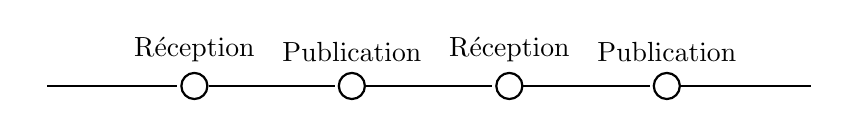
\begin{tikzpicture}[-,>=stealth',shorten >=1pt,auto,node distance=2cm,
  thick,main node/.style={circle,draw,font=\sffamily\Large\bfseries}]

  \node (5) [] {};
  \node[main node] (1) [right of=5, label={above:Réception}] {};
  \node[main node] (2) [right of=1, label={above:Publication}] {};
  \node[main node] (3) [right of=2, label={above:Réception}] {};
  \node[main node] (4) [right of=3, label={above:Publication}] {};
  \node (6) [right of=4] {};

  \path[every node/.style={font=\sffamily\small}]
    (1) edge node [right] {} (2)
    (2) edge node [right] {} (3)
    (3) edge node [right] {} (4)
    (5) edge node [right] {} (1)
    (4) edge node [right] {} (6);
\end{tikzpicture}
\end{frame}

\begin{frame}
\frametitle{Segments}
\framesubtitle{Théorie}
Suite d'opérations effectuées par un \textit{thread} se terminant par une opération de synchronisation
\end{frame}

\begin{frame}
\frametitle{Segments}
\framesubtitle{Pratique}
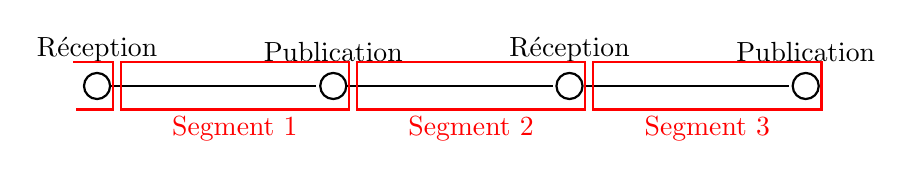
\begin{tikzpicture}[-,>=stealth',shorten >=1pt,auto,node distance=3cm,
  thick,main node/.style={circle,draw,font=\sffamily\Large\bfseries}]

  \node[main node] (1) [label={above:Réception}] {};
  \node[main node] (2) [right of=1, label={above:Publication}] {};
  \node[main node] (3) [right of=2, label={above:Réception}] {};
  \node[main node] (4) [right of=3, label={above:Publication}] {};

  \path[every node/.style={font=\sffamily\small}]
    (1) edge node [right] {} (2)
    (2) edge node [right] {} (3)
    (3) edge node [right] {} (4);
    
    \draw[red] (-0.3, 0.3) -- (0.2, 0.3) -- (0.2, -0.3) -- (-0.3, -0.3);
    \draw[red] (0.3, -0.3) rectangle (3.2, 0.3) node[pos=0.5, below, label={below:Segment 1}] {};
    \draw[red] (3.3, -0.3) rectangle (6.2, 0.3) node[pos=0.5, below, label={below:Segment 2}] {};
    \draw[red] (6.3, -0.3) rectangle (9.2, 0.3) node[pos=0.5, below, label={below:Segment 3}] {};
\end{tikzpicture}
\end{frame}

\begin{frame}
\frametitle{Ordonnancement des segments}
\framesubtitle{Théorie}
\begin{itemize}
\item Un ordre partiel peut être établi en fonction des opérations de synchronisation
\item Dénoté par l'opérateur $\prec$
\end{itemize}
\end{frame}

\begin{frame}
\frametitle{Ordonnancement des segments}
\framesubtitle{Pratique}
\begin{center}
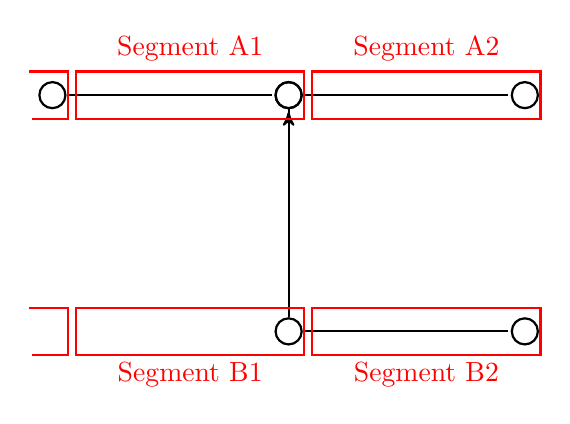
\begin{tikzpicture}[-,>=stealth',shorten >=1pt,auto,node distance=3cm,
  thick,main node/.style={circle,draw,font=\sffamily\Large\bfseries}]

  \node[main node] (1) [] {};
  \node[main node] (2) [right of=1] {};
  \node[main node] (3) [right of=2] {};
  \node[main node] (4) [right of=1] {};
  \node[main node] (5) [right of=5, below of=1] {};
  \node[main node] (6) [right of=6, below of=2] {};

  \path[every node/.style={font=\sffamily\small}]
    (1) edge node [right] {} (2)
    (2) edge node [right] {} (3)
    (4) edge node [right] {} (5)
    (5) edge node [right] {} (6);
    
  \path (5) edge [->] (2);  
  
  \draw[red] (-0.3, 0.3) -- (0.2, 0.3) -- (0.2, -0.3) -- (-0.3, -0.3);
  \draw[red] (0.3, -0.3) rectangle (3.2, 0.3) node[pos=0.5, below, label={[yshift=0.3cm]above:Segment A1}] {};  
  \draw[red] (3.3, -0.3) rectangle (6.2, 0.3) node[pos=0.5, below, label={[yshift=0.3cm]above:Segment A2}] {};
  
  \draw[red] (-0.3, -2.7) -- (0.2, -2.7) -- (0.2, -3.3) -- (-0.3, -3.3);
  \draw[red] (0.3, -3.3) rectangle (3.2, -2.7) node[pos=0.5, below, label={below:Segment B1}] {};  
  \draw[red] (3.3, -3.3) rectangle (6.2, -2.7) node[pos=0.5, below, label={below:Segment B2}] {};
\end{tikzpicture}
\end{center}

\only<2>{
\begin{textblock}{6}(1, 9)
	\textcolor{white}{Segment B1 $\prec$ Segment A2}
\end{textblock}
}
\end{frame}

\begin{frame}
\frametitle{Horloge vectorielle}
\framesubtitle{Théorie}
Structure permettant d'effectuer un ordonnancement partiel des événements dans un système parallèle
\end{frame}

\begin{frame}[shrink=20]
\frametitle{Horloge vectorielle}
\framesubtitle{Pratique}
\begin{center}
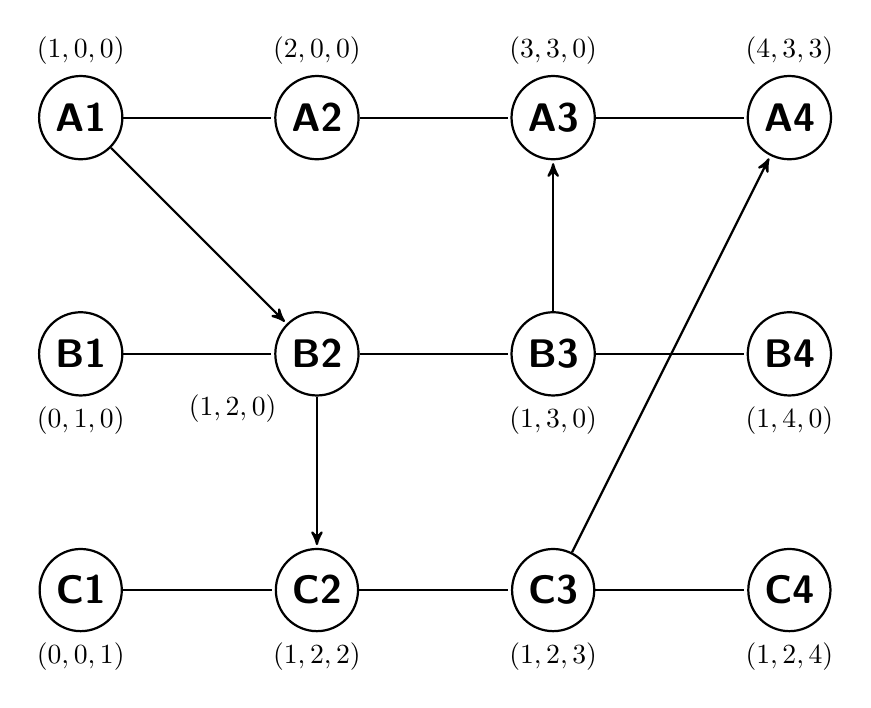
\begin{tikzpicture}[-,>=stealth',shorten >=1pt,auto,node distance=3cm,
  thick,main node/.style={circle,draw,font=\sffamily\Large\bfseries}]

  \node[main node, label=above:{$(1,0,0)$}] (1)  [] {A1};
  \node[main node, label=above:{$(2,0,0)$}] (2)  [right of=1] {A2};
  \node[main node, label=above:{$(3,3,0)$}] (3)  [right of=2] {A3};
  \node[main node, label=above:{$(4,3,3)$}] (4)  [right of=3] {A4};
  
  \node[main node, label=below:{$(0,1,0)$}] (5)  [below of=1] {B1};
  \node[main node, label=below left:{$(1,2,0)$}] (6)  [right of=5] {B2};
  \node[main node, label=below:{$(1,3,0)$}] (7)  [right of=6] {B3};
  \node[main node, label=below:{$(1,4,0)$}] (8)  [right of=7] {B4};
  
  \node[main node, label=below:{$(0,0,1)$}] (9)  [below of=5] {C1};
  \node[main node, label=below:{$(1,2,2)$}] (10) [right of=9] {C2};
  \node[main node, label=below:{$(1,2,3)$}] (11) [right of=10] {C3};
  \node[main node, label=below:{$(1,2,4)$}] (12) [right of=11] {C4};

  \path[every node/.style={font=\sffamily\small}]
    (1) edge node [right] {} (2)
    (2) edge node [right] {} (3)
    (3) edge node [right] {} (4)
    (5) edge node [right] {} (6)
    (6) edge node [right] {} (7)
    (7) edge node [right] {} (8)
    (9) edge node [right] {} (10)
    (10) edge node [right] {} (11)
    (11) edge node [right] {} (12);
  
  \path (1) edge [->] (6);
  \path (6) edge [->] (10);
  \path (11) edge [->] (4);
  \path (7) edge [->] (3);
\end{tikzpicture}
\end{center}
\end{frame}


\begin{frame}
\frametitle{Conditions de course}
\begin{columns}
    \begin{column}{0.5\textwidth}
Deux accès mémoire dont au moins un est une écriture et qui pourraient être exécutées simultanément sans connaissance des manipulations effectuées par l'autre \textit{thread} 
    \end{column}
    \begin{column}{0.5\textwidth}
\begin{center}
\begin{tikzpicture}[-,>=stealth',shorten >=1pt,auto,node distance=2.5cm,
  thick,main node/.style={circle,draw,font=\sffamily\Large\bfseries}]

  \node (1) [label={above:$T$}] {};
  \node[main node] (2) [below of=1, label={above left:x=1}, label={below left:(2, 2)}] {};
  \node (3) [below of=2] {};
  
  \node (4) [right of=1, label={above:$T^{\prime}$}] {};
  \node[main node] (5) [below of=4, label={above right:if(x==1)}, label={below right:(2, 2)}] {};
  \node (6) [below of=5] {};

  \path[every node/.style={font=\sffamily\small}]
    (1) edge node [right] {} (2)
    (2) edge node [right] {} (3)
    (4) edge node [right] {} (5)
    (5) edge node [right] {} (6);
\end{tikzpicture}
\end{center}
    \end{column}
\end{columns}
\end{frame}

\subsection{Algorithme}
\begin{frame}
\frametitle{Algorithme}
\framesubtitle{Équations}
Il y a une condition de course entre un segment $S$ et un segment $S^{\prime}$ si:
\begin{itemize}
\item[1.]  $V_{S}(T) \geq V_{S^{\prime}}(T)$ et $V_{S^{\prime}}(T^{\prime}) \geq V_{S}(T^{\prime})$
\item[2.]  $[R_{S} \cup W_{S}] \cap W_{S^{\prime}} \neq \emptyset$ ou $[R_{S^{\prime}} \cup W_{S^{\prime}}] \cap W_{S} \neq \emptyset$
\end{itemize}
\end{frame}

\begin{frame}
\frametitle{Algorithme}
\framesubtitle{Pratique}
\begin{columns}
    \begin{column}{0.5\textwidth}
\begin{itemize}
\item[\checkmark] $V_{S}(T) \geq V_{S^{\prime}}(T)$
\item[\checkmark]<2-> $V_{S^{\prime}}(T^{\prime}) \geq V_{S}(T^{\prime})$
\item[\checkmark]<3-> $[R_{S^{\prime}} \cup W_{S^{\prime}}] \cap W_{S} \neq \emptyset$
\end{itemize}
    \end{column}
    \begin{column}{0.5\textwidth}
\begin{center}
\begin{tikzpicture}[-,>=stealth',shorten >=1pt,auto,node distance=2.5cm,
  thick,main node/.style={circle,draw,font=\sffamily\Large\bfseries}]

  \node (1) [] {};
  \node[main node] (2) [below of=1, label={above left:x=1}, label={below left:(2, 2)}] {};
  \node (3) [below of=2] {};
  
  \node (4) [right of=1] {};
  \node[main node] (5) [below of=4, label={above right:if(x==1)}, label={below right:(2, 2)}] {};
  \node (6) [below of=5] {};

  \path[every node/.style={font=\sffamily\small}]
    (1) edge node [right] {} (2)
    (2) edge node [right] {} (3)
    (4) edge node [right] {} (5)
    (5) edge node [right] {} (6);
\end{tikzpicture}
\end{center}
    \end{column}
\end{columns}
\end{frame}

\section{Ensemble de verrous}
\subsection{Idée}
\begin{frame}
\frametitle{Idée}
Un programme parallèle sans condition de course respecte toujours une saine discipline de verrouillage des structures partagées
\end{frame}

\subsection{Algorithme}
\begin{frame}
\frametitle{Algorithme}
\framesubtitle{Ébauche}
But: S'assurer que toute structure partagée soit protégée par un verrou
\end{frame}

\begin{frame}
\frametitle{Algorithme}
\framesubtitle{Ébauche}
\begin{algorithm}[H]
 Verrous(\textit{T}) = Ensemble de verrous acquis par un \textit{thread T}\;
 C(\textit{v}) = verrous possibles pour une variable \textit{v}\;
 
 \For{Toute variable partagé \textit{v}}{
 C(\textit{v}) = tous les verrous présents dans l'application
 }
 
 \For{Tout accès à une variable partagé \textit{v}}{
 C(\textit{v}) = C(\textit{v}) $\cap$ Verrous(\textit{T})\;
 \If{C(\textit{v}) == \{\}}{
   Condition de course détectée 
 }
 }
\end{algorithm}
\end{frame}

\begin{frame}[fragile]
\frametitle{Algorithme}
\framesubtitle{Ébauche}
\begin{columns}
    \begin{column}{0.48\textwidth}
        \begin{lstlisting}
Mutex1.lock();
v = v + 1;
Mutex1.unlock();
Mutex2.lock();
v = v + 1;
Mutex2.unlock();
\end{lstlisting}
\only<1>{
\begin{textblock}{5}(5.75, 6.47)
	 \scalebox{1.5}{$\Lleftarrow$}
\end{textblock}
}
\only<2>{
\begin{textblock}{5}(5.75, 7.33)
	 \scalebox{1.5}{$\Lleftarrow$}
\end{textblock}
}
\only<3>{
\begin{textblock}{5}(5.75, 8)
	 \scalebox{1.5}{$\Lleftarrow$}
\end{textblock}
}
\only<4>{
\begin{textblock}{5}(5.75, 8.91)
	 \scalebox{1.5}{$\Lleftarrow$}
\end{textblock}
}
\only<5>{
\begin{textblock}{5}(5.75, 9.7)
	 \scalebox{1.5}{$\Lleftarrow$}
\end{textblock}
}
\only<6>{
\begin{textblock}{5}(5.75, 10.35)
	 \scalebox{1.5}{$\Lleftarrow$}
\end{textblock}
}
\only<7>{
\begin{textblock}{5}(5.75, 11.3)
	 \scalebox{1.5}{$\Lleftarrow$}
\end{textblock}
}
    \end{column}
    \begin{column}{0.55\textwidth}
        \begin{tabular}{ | c | c | }
  \hline
  Verrous & C(\textit{v}) \\
  \hline
  \{\} & \{Mutex1, Mutex2\} \\
  \hline
  \onslide<2->{\{Mutex1\} & \{Mutex1, Mutex2\}} \\
  \hline
  \onslide<3->{\{Mutex1\} & \{Mutex1\}} \\
  \hline
  \onslide<4->{\{\} & \{Mutex1\}} \\
  \hline
  \onslide<5->{\{Mutex2\} & \{Mutex1\}} \\
  \hline
  \onslide<6->{\{Mutex2\} & \{Mutex1\}} \\
  \hline
  \onslide<7->{\{\} & \{\}} \\
  \hline
\end{tabular}
    \end{column}
\end{columns}
\end{frame}

\begin{frame}
\frametitle{Algorithme}
\framesubtitle{Ébauche}
Trois problèmes de l'algorithme précédent
\begin{itemize}
\item Initialisation
\item Structure seulement en lecture
\item Verrou lecture-écriture
\end{itemize}
\end{frame}

\begin{frame}
\frametitle{Algorithme}
\framesubtitle{Raffinement}
\begin{center}
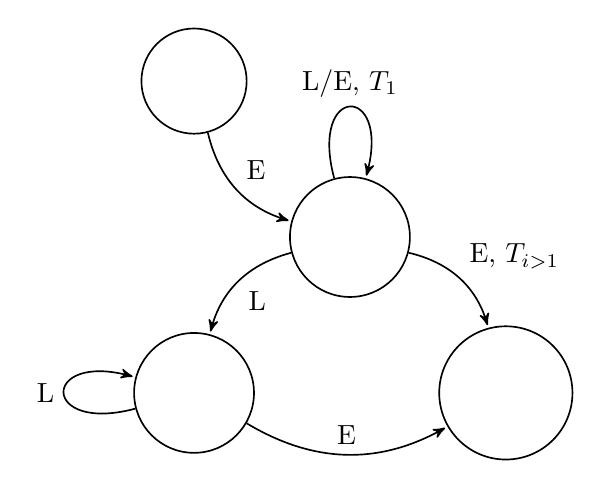
\begin{tikzpicture}[->,>=stealth',shorten >=1pt,auto,node distance=2.8cm,
                    semithick]
  \tikzstyle{every state}=[text=white]

  \node[state]         (A)                    {Exclusif};
  \node[state]         (B) [above left of=A] {Vierge};
  \node[state]         (D) [below left of=A] {Partagé};
  \node[state]         (C) [below right of=A, text width=1.2cm] {Partagé-Modifié};

  \path (A) edge [bend right] node {L} (D)
            edge [bend left]  node {E, $T_{i>1}$} (C)
            edge [loop above]  node {L/E, $T_{1}$} (A)
        (B) edge [bend right] node {E} (A)
        (D) edge [bend right] node {E} (C)
        (D) edge [loop left]  node {L} (B)
        ;
\end{tikzpicture}
\end{center}
\end{frame}

\begin{frame}[shrink=25]
\frametitle{Algorithme}
\framesubtitle{Raffinement}
\begin{algorithm}[H]
 Verrous(\textit{T}) = Ensemble de verrous acquis par un \textit{thread T}\;
 Verrous\_É(\textit{T}) = Ensemble de verrous en mode écriture acquis par un \textit{thread T}\;
 C(\textit{v}) = verrous possibles pour une variable \textit{v}\;
 
 \For{Toute variable partagé \textit{v}}{
 C(\textit{v}) = tous les verrous présents dans l'application
 }
 
 \For{Toute lecture d'une variable partagé \textit{v}}{
 C(\textit{v}) = C(\textit{v}) $\cap$ Verrous(\textit{T})\;
 \If{C(\textit{v}) == \{\}}{
   Condition de course détectée 
 }
 }
 
 \For{Toute écriture d'une variable partagé \textit{v}}{
 C(\textit{v}) = C(\textit{v}) $\cap$ Verrous\_É(\textit{T})\;
 \If{C(\textit{v}) == \{\}}{
   Condition de course détectée 
 }
 }
\end{algorithm}
\end{frame}

\section{Comparaison}
\subsection{Implémentation}
\begin{frame}
\frametitle{Implémentation}
\framesubtitle{Instrumentation}
\begin{itemize}
\item Recompilation dynamique de binaires
\item Fait souvent appel à de la \textit{shadow memory}
\item Ne diffère que dans les instructions visés
\end{itemize}
\end{frame}

\begin{frame}[fragile]
\frametitle{Implémentation}
\framesubtitle{Annotations}
Pour aider le processus de détections, les outils offrent souvent la possibilité d'annoter un programe. Par exemple: 
\begin{columns}
    \begin{column}{0.6\textwidth}
    \begin{center}
ThreadSanitizer  
    \end{center}
    \footnotesize{
    \begin{lstlisting}
ANNOTATE_IGNORE_WRITES_BEGIN
ANNOTATE_IGNORE_WRITES_END
ANNOTATE_CONDVAR_LOCK_WAIT(cv, mu)
ANNOTATE_BENIGN_RACE(ptr)
\end{lstlisting}}
    \end{column}
    \begin{column}{0.4\textwidth}
    \begin{center}
Eraser    
    \end{center}
    \footnotesize{
    \begin{lstlisting}
EraserReadLock(lock)
EraserReadUnLock(lock)
EraserWriteLock(lock)
EraserWriteUnLock(lock)
\end{lstlisting}}
    \end{column}
\end{columns}
\end{frame}

\subsection{Conditions de course détectées}
\begin{frame}[fragile]
\frametitle{Cas non détecté par arrivé-avant}
\begin{columns}
    \begin{column}{0.5\textwidth}
    \begin{center}
Thread 1  
    \end{center}
    \begin{lstlisting}
  Y += 1;
  Mutex.lock();
  V += 1;
  Mutex.unlock();
\end{lstlisting}
    \end{column}
    \begin{column}{0.5\textwidth}
    \begin{center}
Thread 2    
    \end{center}
    \begin{lstlisting}
  Mutex.lock();
  V += 1;
  Mutex.unlock();
  Y += 1;
\end{lstlisting}
    \end{column}
\end{columns}
\end{frame}

\begin{frame}[fragile]
\frametitle{Cas non détecté par ensemble de verrous}
\begin{lstlisting}
int main() {
  int X = 0;
  std::thread T([&](){ X++; });
  X += 42;
  T.join();
}
\end{lstlisting}
\end{frame}

\begin{frame}
\frametitle{Résumé}
Les faits importants à retenir:
\begin{itemize}
\item Arrivé-avant détecte moins de conditions de course que l'ensemble de verrous
\item L'ensemble de verrou peut produire des faux positifs contrairement à arrivé-avant
\item Les deux algorithmes peuvent produire des faux négatifs
\end{itemize}
\end{frame}

\section{Conclusion}
\begin{frame}
\frametitle{Conclusion}
La plupart des outils de détection de condition de courses implémentent une variation ou une combinaison des algorithmes présentés.
\end{frame}

\end{document}